\chapter{Introduction}

Our \glspl{ECU} are based on ARM Cortex-M1/M3 controllers. Both of them became recently available as an \gls{IP}-package for Xilinx based \glspl{FPGA}.
By using a common hardware base and a common software middleware we were able to streamline the development of the control-software which enables a faster development process for new applications and reduces the overhead of their functional verification.
 
Brief overview, problem statement and final outcome.

\section{Design Overview}

The assumed system consists of three regular separate control units that are connected through a communication link. Figure \ref{fig:basicDesign} shows the basic components of the assumed design.

\begin{figure}[h!]
    \centering
    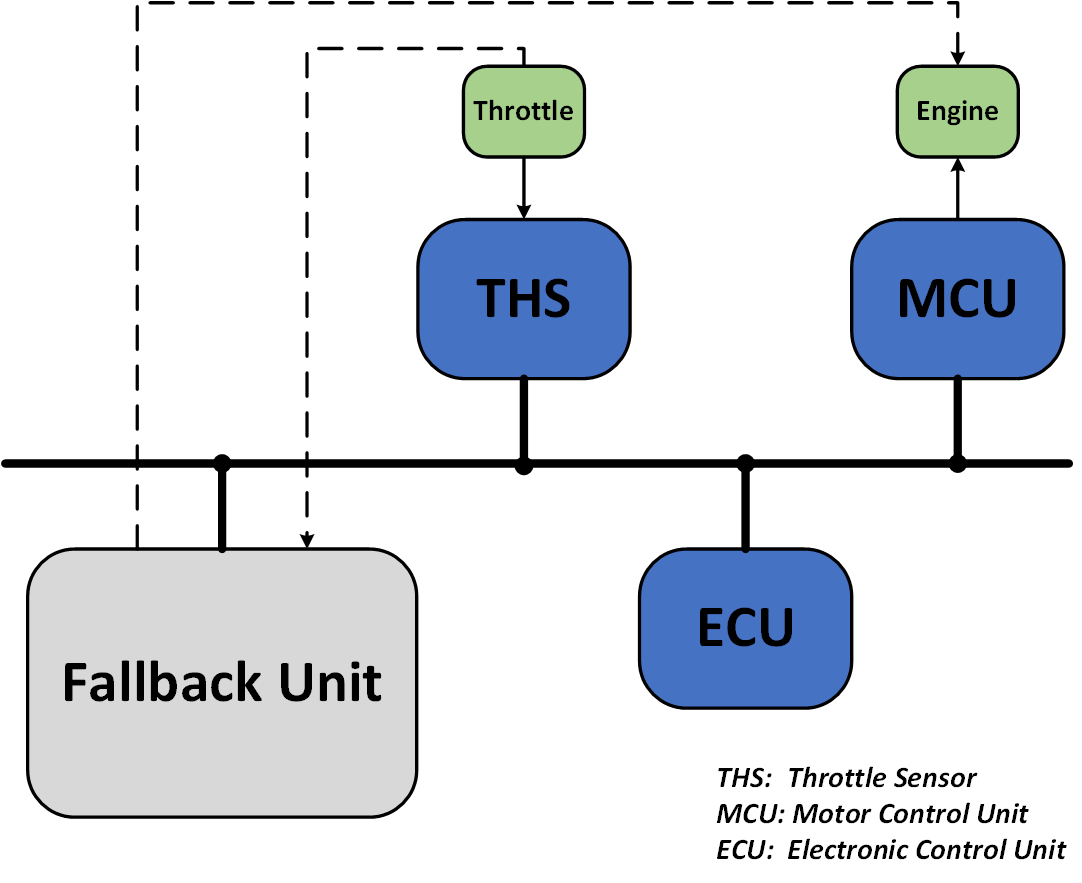
\includegraphics[width=0.75\textwidth]{figures/basic_design.png}
    \caption{Basic concept for Failsafe ECU}\label{fig:basicDesign}
\end{figure}

The realized scenario reads a throttle position and controls an engine after some data conversion. The \gls{ECU} is responsible for gathering the throttle position data, measured and provided by the \gls{THS}. After the \gls{ECU} converts the throttle position data into engine control data, it forwards these data to the \gls{MCU}, which is responsible for controlling the engine. A fourth unit acts as a fallback unit in case of a failure of one of the regular control units. This fallback unit is realized by using \gls{PR} in an \gls{FPGA}. Figure \ref{fig:sequenceNormalOp} displays a sequence diagram assuming normal operation. In this case, the fallback unit doesn't have to perform any active functionality, it just has to passively monitor the data transfer on the communication link to detect possible errors.

\begin{figure}[h!]
    \centering
    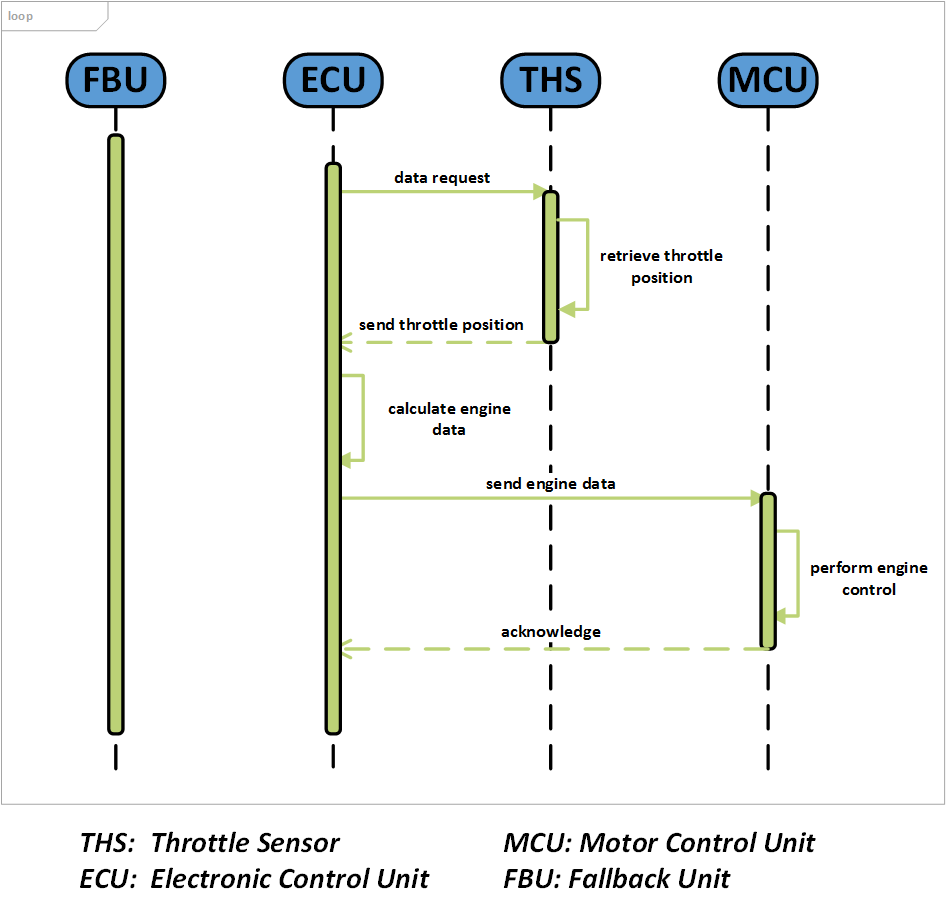
\includegraphics[width=\textwidth]{figures/sequence_normal_op.png}
    \caption{Sequence diagram for normal operation}\label{fig:sequenceNormalOp}
\end{figure}

The fallback unit has to monitor all transferred data on the bus and detect any failures (e.g. timeout, error flags, ...). 
Once an error is detected, a certain partial reconfiguration is triggered by the bus monitor module, which is part of the fallback unit. 
After the reconfiguration is finished, the fallback unit completely takes over the functionality of the faulty component. 
Due to the fail silent assumption, the faulty device will not affect the behaviour of the system. 
Figure \ref{fig:sequenceMCUFailure} shows a sequence diagram including a faulty \gls{MCU}. 
The bus monitor detects that the \gls{MCU} is running into a timeout and triggers a \gls{PR} to take over its functionality. 
After finishing the reconfiguration, normal operation takes over again (see figure \ref{fig:sequenceNormalOp}), but the fallback unit serves as \gls{MCU} now.

\begin{figure}[h!]
    \centering
    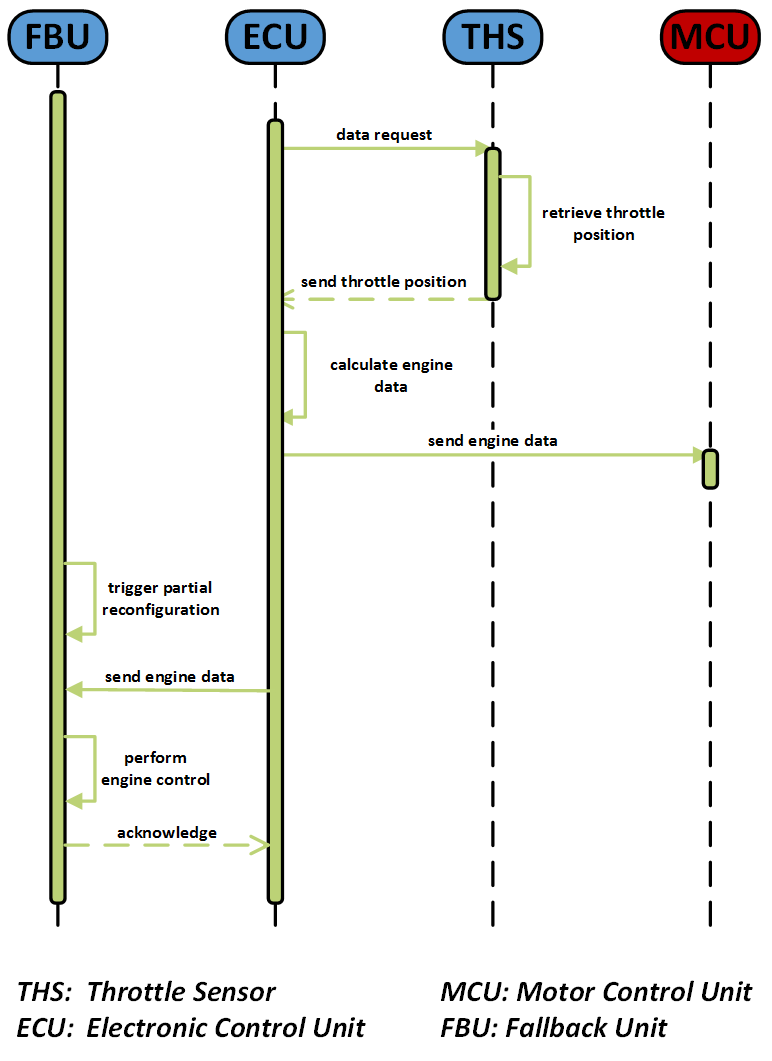
\includegraphics[width=\textwidth]{figures/sequence_mcu_fail.png}
    \caption{Sequence diagram for \gls{MCU} failure}\label{fig:sequenceMCUFailure}
\end{figure}

\section{Required tools, \glspl{IP} and packages}
TODO: licenses
\begin{itemize}
    \item Vivado 2018.3
    \item Vivado 2018.2
    \item uVision 5 (Windows only)
    \item ARM Keil (Windows only)
    \item ARM Cortex M1 IP for Vivado
    \item UART IP by Martin Mosbeck
    \item ARM Mbed OS
\end{itemize}
